\chapter{Approach}\label{sec:approach}

\section{Considerations and Challenges}\label{sec:considerations}

First of all, working with special hardware like the DVS requires a different approach to handling and processing the data. Using normal cameras, naturally conventional vision algorithms are based on the analysis of frames. In order to make use of the asynchronous behaviour an image-based approach is not feasible for maintaining the high temporal resolution, i.e. the algorithm had to make use of the event-based behaviour of the DVS.
Another property to keep in mind with the DVS is the fact that data is only provided if there is a change in illumination, e.g. motion. This means that a static input will not generate significant output.
A limitation to keep in mind is the low spatial resolution. This makes it infeasible to detect smaller features which high resolution cameras are able to. Thus the low resolution also introduces a higher uncertainty towards visual cues in comparison to conventional cameras.
As explained in the introduction, the sampling frequency i.e. the temporal resolution of the DVS varies. Therefore it was necessary to measure what frequencies could be handled by the DVS especially in respect to our drone flight scenario.

\section{Preparation}\label{sec:preparation}

In this paragraph the necessary preparations before the implementation of the tracking algorithm are discussed. These comprise of writing a driver interface in C++ to the DVS as well as building a set of active markers.

\subsection{C++ interface to the DVS}\label{sec:interface}

The framework provided with the DVS called jAER\footnote{http://sourceforge.net/apps/trac/jaer} is completely written in Java as well as the tracking algorithm developed by \cite{Matthias}. Since we wanted to implement our approach in C++ due to performance and portability considerations (e.g. to embedded systems) it was necessary to write a driver interface to the DVS first. Thesycon\footnote{http://www.thesycon.de/eng/home.shtml}, the provider of the USB device driver, already offers a framework to communicate with their driver. This was employed to pull the event data from the DVS. Similar to jAER, the events are wrapped up in packets of several events. The packet size depends on the junk of data which arrives at once from the USB . This not only makes sense as the data arrive in chunks of up to several hundred events from the USB buffer; packet-based processing is furthermore advantageous for certain operations, e.g. if they are computationally costly and single events do not provide enough relevant information to be processed individually. 

\subsection{LED markers}\label{sec:leds}

In order to build a set of blinking LEDs with different frequencies we used the bronze board\footnote{http://www.ini.uzh.ch/~tobi/wiki/doku.php?id=dig:uc} from INI which is based on an AVR32. A USB interface provides the means for simple programming and communication with the microcontroller. Although a less powerful microprocessor would have been sufficient, a high number of independent Pulse-Width-Modulation (PWM) drivers was an important property in order to drive several LEDs with different frequencies. The bronze board has 7 PWM drivers, from which 5 are free to use.  An already existing C code example was taken and adapted to our needs. Additionally, a python script provided the means of remotely adjusting the PWM via USB. 
The choice of LEDs was important, since they should be well visible. The ideal LED for our project would provide high illuminance and a wide emission angle. Since the DVS is very sensitive to the infra-red spectrum, we decided to go for infra-red LEDs[type hint]. We decided to attach four LEDs to our quadrotor which is the minimum number to estimate the pose in 3D space.


\section{The tracking algorithm}\label{sec:tracking}

The following paragraphs describe the separate steps of the tracking algorithm we developed. Figure \ref{img:process_diag} provides an overview over the stages described in the following sections. The approach designed by \cite{Matthias} works on a more general level assuming the blinking pattern to be previously unknown. 
As we wanted to design our algorithm for a specific task, namely tracking a helicopter, these constraints gave us the opportunity to simplify the algorithm. In our setup we would be tracking specific LEDs attached to a helicopter, of which we already knew the blinking pattern, as well as the position towards each other. While in \cite{Matthias} the algorithm starts by finding high-activity clusters, denoting the position of a blinking LED, we decided to take a different approach. Fixing different frequencies to our LEDs allowed us to first filter frequency space to get rid of background noise and extract the relevant information. The signals we used for this resemble a square wave with 50\% duty rate. The following section describes the filtering process, as well as the choice of frequencies.


\begin{figure}[h]
     \centering
     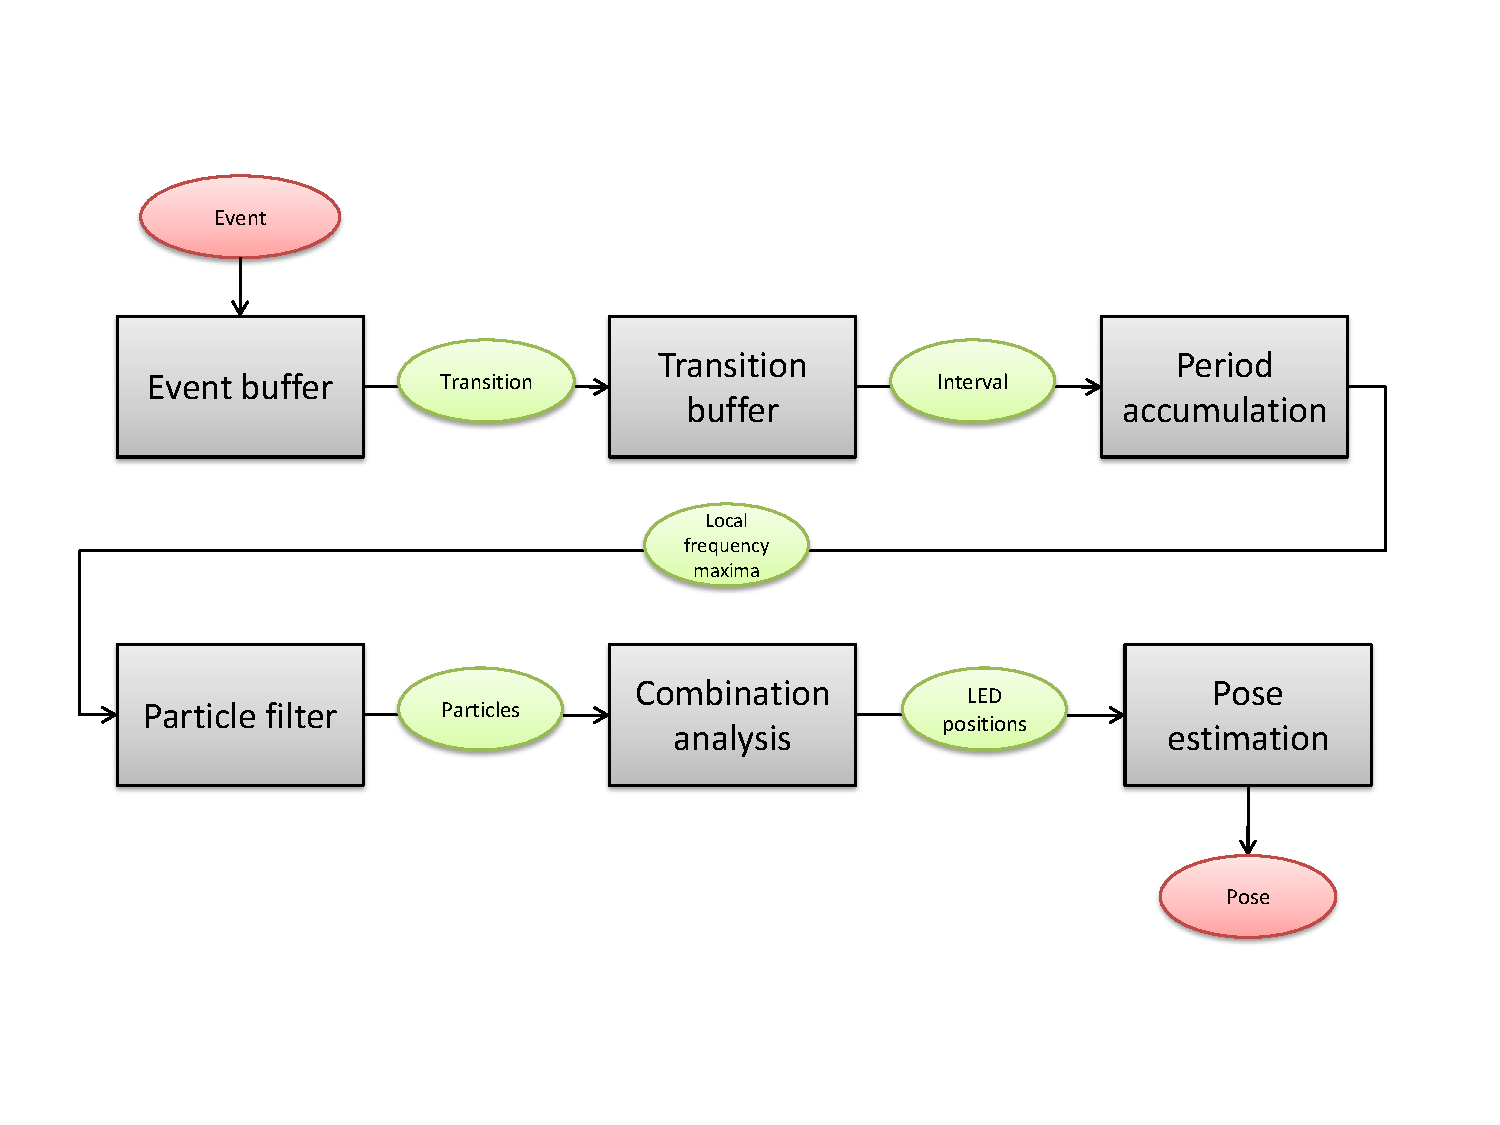
\includegraphics[width=1.0\textwidth]{img/process_diag.pdf}
     \caption{Sequential diagram of the processing stages. The boxes show the different processing stages while the circles denote the different data containers. }
     \label{img:process_diag}
\end{figure}


\subsection{Frequency filter}\label{sec:frequencyfilter}

There are two main challenges to consider in frequency analysis:
\begin{itemize}
\item The correct measurement of frequencies
\item The influence of background noise in frequency measurement
\end{itemize}

Having static LEDs in the camera's "`image"' the straight-forward approach of measuring the inter-spike-intervals\footnote{A term often used in neuroscience to describe the time interval between two consecutive spikes on the same neuron, here used for a pixel.} (ISI) would be evident as changes of LED state(from on to off or vice versa) should generate consecutive events of different polarity and thus yield to the signal period. This approach should also work for moving LEDs as long as the frequencies are high and the LED velocity is low enough, so that consecutive state changes overlap to generate events on the same pixels. Since this has shown to be true for the maximum possible velocity of the quadrotor towards the camera, we went for this approach.
In order to address the influence of background noise we needed to find out what ISIs were usually generated by it. Therefore, we recorded data over several scenarios with the DVS by moving it over our set of pulsed LEDs fixed to the ground. This included different distances and speeds, as well as varying backgrounds. Thereby, background containing many edges would generate a considerably higher amount of events than a uniform backgrounds (e.g. a white wall). Evaluating the different data on a frequency histogram we found that most of the movement induced background noise generates frequencies up to around 500 Hz (\ref{img:hist_motion}). Thus, to make our LEDs well distinguishable they needed to be pulsed with frequencies above this limit. Additionally to the lower boundary an upper limit also needed to be considered as the sampling accuracy of the DVS drops with higher frequencies \cite{Matthias}. Furthermore, the spacing between the frequencies was also important in order to prevent inaccurate measurement to deliver false detections and thus keep our markers well distinguishable. Last but not least, the frequencies should not be multiples of each other to ensure robustness towards occasional data loss (i.e. if a state change of the LED is missed the period will not be confused with the one of another LED). Experiments showed frequencies of 740, 1030, 1320 and 1610 Hz to work well.

\begin{figure}[h]
     \centering
     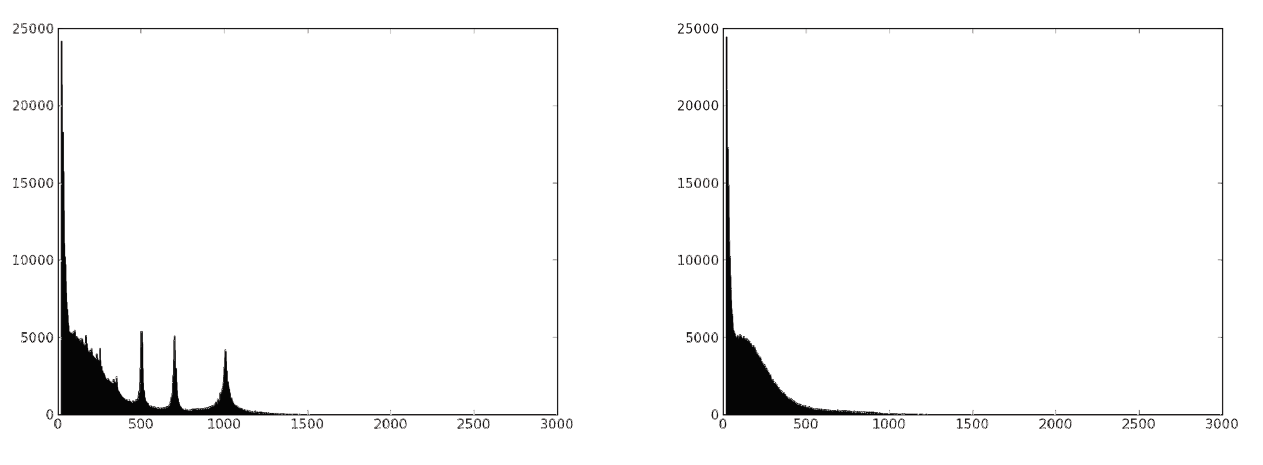
\includegraphics[width=1.0\textwidth]{img/hist_motion.png}
     \caption{Frequency histograms for a DVS recording with high motion. Left: Includes three LEDs pulsed at 500, 700 and 1000 Hz. Right: Without LEDs. }
     \label{img:hist_motion}
\end{figure}


\subsection{Frequency period estimation}\label{sec:periodestimation}

Following the approach of using ISIs for period estimation, where an event denotes a rising or falling edge of the signal, these needed to be measured first for each pixel. As we found, two consecutive events on a pixel excited by a blinking LED did not always have different polarity. Instead, several successive events of the same polarity are generated. This can be related to the high sensitivity of the DVS as well as the non-uniform illumination coming from an LED over time. Therefore, it was necessary to observe consecutive events and note a state transition, whenever they were of different polarity. This provided us with two kinds of transitions, namely from positive to negative polarity or vice versa. Two consecutive transitions of the same type would then yield the signal period. 
In order to keep track of the latest events on a per pixel level, we use a 2D array resembling the pixel space of the DVS, where only the latest event for each pixel is stored.  Before inserting a new event into the array, its type is compared to the preceding event.  If their polarities differ a transition is generated. The values contained in a transition are similar to events:

\begin{itemize}
	\item Position \{x,y\}
	\item Type \{on-to-off \textbar\ off-to-on\}
	\item Time stamp \{t\}
\end{itemize}

Like the previous step each transition is mapped onto a 2D array with pixel space resolution. To keep track of each transition type two 2D-arrays are used to store the latest transitions. Following our previous assumption, before insertion of a new transition the time interval to its predecessor is now measured. This provides a period and thus a certain frequency estimate. An interval is stored with:

\begin{itemize}
	\item Position \{x,y\}
	\item Time stamp \{t\}
	\item Time interval \{\delta t\}
\end{itemize}

\subsection{Period accumulation}\label{sec:frequencyaccumulation}

In order to find the relevant frequencies each measurement is weighted with a Gaussian according to its distance to each of the frequencies we want to find. 
This provides us with different likelihoods (according to the magnitude of weight) of having found a relevant frequency. The weights are stored in a weight map, again a 2D array of pixel-space resolution. Figure \ref{img:dvs_weights} shows the raw DVS output and the aggregated weight map over all frequencies. In order to increase the robustness and to avoid noise induced weights to influence our frequency filter it was important to gather several weights per pixel to support the hypothesis of having found a pulsed signal. Since we are interested in extracting four distinct signals a weight map for each needs to be maintained. Each pixel in the map gathers the sum of weights measured during a certain time. An interval of 10 ms during weights are gathered provided feasible results. The most likely position of a certain LED is then estimated by taking the pixels with the most support into account, i.e. the ones with the highest weight.  Therefore a set of local maxima in the weight map needs to be maintained. We also introduced a minimum distance between maxima to allow only one maximum per LED to be found. A distance of 15 pixels was chosen, as this is larger than the usual area covered by a single LED. The number of local maxima to maintain was set to three, as experiments showed additional maxima to have a comparably much lower significance. For the Gaussian weighting we allowed a standard deviation of 30 Hz.

\begin{figure}[h]
     \centering
     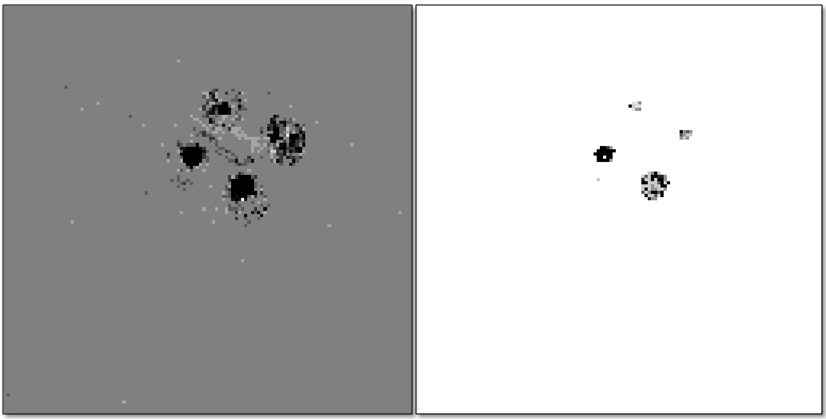
\includegraphics[width=1.0\textwidth]{img/dvs_weights.png}
     \caption{Left: The raw DVS output. Right: An aggregation of all weight maps. The darkness of the pixels indicates the magnitude of weight.}
     \label{img:dvs_weights}
\end{figure}

\section{LED position estimation}\label{sec:positionestimation}

So far the local maxima provide us different hypothesis of the location of each LED. This gives us only a snapshot in time of the current most likely locations though. In order to increase robustness by observing the positions over time as well as taking motion of the quadcopter into account we applied a particle filter. This technique is widely used in robotics for state estimation. The following paragraph describes our application this approach.


\subsection{Particle filter}\label{sec:particlefilter}

So far each evaluation of local maxima provides three hypotheses denoting the possible marker positions. Each hypothesis is now used to update a particle filter. For each signal we want to find, there is a particle filter maintained with a fixed set of particles. Such a particle stores the following values:

\begin{itemize}
	\item Position \{x,y\}
	\item Time stamp \{t\}
	\item Uncertainty \{\sigma \}
	\item Weight	\{w\}
\end{itemize}

The position in pixel-space thereby has sub-pixel resolution. The uncertainty of the particle denotes the possible radius in pixels in which the LED can move in time representing our motion model. Thus the uncertainty of a particle grows in time, according to the maximum possible speed an LED can move in image space. If the uncertainty reaches a certain threshold, i.e. the uncertainty is too high, the particle expires and is deleted. The weight denotes the amount of support a particle has and the time stamp marks the time of its creation.\\

Initially, the particle filter is empty. For every new hypothesis a candidate particle is created. Thereby, the position and weight are inherited from the local weight maxima while the uncertainty is set to a default value of 2 pixels. The latest incoming event marks the time of particle creation.  Each candidate can now become a new particle in the filter or is merged with an existing one. Candidates are thus compared to existing particles to see if their position falls into the uncertainty radius of an existing particle. In this case, and under the assumption of our motion model, this would mean that the candidate indicates a valid consecutive position in time of an LED. If no existing particle can be updated, the candidate is inserted into the filter while replacing the oldest particle if the filter is full.
During merging the uncertainties decide upon the contribution of the two particles to the new one created. The new position is linearly interpolated. Similarly, the new weight is a summation of particle values weighted by their uncertainty. Finally, the new uncertainty is calculated by a multiplication of Gaussians.

\subsection{Extracting LED positions}\label{sec:ledpositions}

In this final step we need to decide on the definitive positions of the four LEDs. So far we have a particle filter for each LED with a number of particles denoting the most likely positions for the LEDs. A straight-forward approach would choose the particle with the highest weight from each filter, i.e. the particle with the highest support. Unfortunately though, we found that the frequencies we used were still close enough to be ambiguous for frequency estimation. Thus, apart from random noise, close-by frequencies tended to have particles of different frequency on the same LED position. This required then, to find the best valid combination of particles where they all had distinct positions and thus should resemble our marker positions. The significance of a valid combination was thereby found by multiplying the particle weights.
In order to solve this combinational problem a recursive function is used to traverse all the different combinations. Since this combinatorial problem implies many recursions, becoming computationally costly, we introduced some heuristics to reduce the number of recursions. First, each particle filter was sorted in descending order according to particle weights. This should favour traversing the most significant combinations early. In addition, since we were only interested in a limited number of most likely combinations, after finding enough hypotheses a branch would only be expanded if its score was bigger than the least significant score of the hypotheses found so far. For choosing the right combination, we took the straight forward approach of selecting the one with the highest score. 

\subsection{Pose estimation}\label{sec:poseestimation}

Given the marker positions, we were now able to estimate the relative pose of the helicopter to the camera. We used an existing algorithm from OpenCV\footnote{http://opencv.org/} for that purpose. Given the feature points in the objects reference frame, the correspondent points in image space, as well as the intrinsic camera parameters and its distortion values, the algorithm computes a rotation and translation of the object towards the camera reference frame.

\subsection{Discussion}\label{sec:approach_discussion}

As mentioned in section \ref{sec:ledpositions}, the inaccuracy of frequency estimation caused several frequencies detected on the ISIs generated by the same LED. It can therefore also happen that positions jump for a short time. Although this happens only on very few occasions further measures need to be taken to improve robustness. Another problem in the approach is the fact that the local maxima, which come from a single pixel, are taken to update a particle. Since an LED usually produces a blob comprising several pixels on the camera, maxima tend to jump between different pixels of this blob, which gives the particles and thus also the final LED positions an oscillating behavior.